\documentclass[journal, table]{IEEEtran}
\usepackage[utf8]{inputenc}
\usepackage[english, spanish]{babel}
\usepackage[sorting=none]{biblatex}
\bibliography{ref.bib}

\usepackage{amsmath, amsfonts, amsthm, amssymb, mathtools}
\usepackage{hyperref, url}
\usepackage[dvipsnames]{xcolor}
\usepackage{fancyhdr, last page}
\usepackage{siunitx}
\usepackage{graphicx}
\usepackage[affil-sl]{authblk}
\usepackage{anyfontsize}
\usepackage{graphicx}
\usepackage{subfigure}
\usepackage{csquotes}
\usepackage{float}
\usepackage{svg}
\usepackage{tabularx, ragged2e, booktabs}
\usepackage{siunitx}
\usepackage[spanish]{cleveref}
\AtBeginDocument{\decimalpoint}
\graphicspath{{./images}}

\hypersetup{
    colorlinks=true,
    linkcolor=black,
    urlcolor=blue,
    pdftitle={Filiform Lab - JLBA}
}
\urlstyle{same}
\sisetup{separate-uncertainty}

\begin{document}

\title{}

\author[*]{Laura Herrera
    \thanks{Laura Herrera: 20212107011}}
\author[*]{Bryan Martínez
    \thanks{Bryan Martínez: 20212107008}}
\author[*]{Julian Avila
    \thanks{Julian Avila: 20212107030}}
\author[*]{Juan Acuña
    \thanks{Juan Acuña: 20212107034}}


\affil[*]{Programa Académico de Fisica\\
Universidad Distrital Francisco José de Caldas}

\markboth{}
{Shell \MakeLowercase{\textit{et al.}}: Bare Demo of IEEEtran.cls for IEEE Journals}

\maketitle

\selectlanguage{english}
\begin{abstract}
The Millikan experiment is proposed to determine the charge of the electron.
To achieve this, the falling velocity of an oil drop is measured under the
influence of gravity, buoyant force, and friction. Subsequently, a potential
difference is applied between plates, causing the drop to rise, and this ascent
velocity is measured.
The software \emph{Tracker} was used in this experiment to determine these
velocities.
Once the velocities are measured, an analysis of the involved forces is
performed to calculate the radius and charge of each drop.
A total of 20 drops were recorded, and using a code in \emph{Julia},
the greatest common divisor of the obtained charges was determined.
Finally, the charge of the electron was estimated to be approximately
\( e^{-} \approx \qty{1.50e-19}{C} \).
\end{abstract}

\begin{IEEEkeywords}
Millikan Experiment, Elementary Charge, Quantization.
\end{IEEEkeywords}

\selectlanguage{spanish}
\begin{abstract}
Se propone realizar el experimento de Millikan para determinar la carga del
electrón.
Para ello, se mide la velocidad de caída de una gota de aceite bajo la
influencia de la gravedad, la fuerza de empuje y la fricción.
Posteriormente, se aplica una diferencia de potencial entre placas, lo que
provoca una velocidad de ascenso de la gota, la cual se mide.
En esta práctica se utilizó el software \emph{Tracker} para determinar
dichas velocidades.
Una vez medidas las velocidades, se realiza un análisis de las fuerzas
involucradas para calcular el radio y la carga de cada gota.
Se registraron un total de 20 gotas, y mediante un código en \emph{Julia} se
determinó el mínimo común divisor de las cargas obtenidas.
Finalmente, se estimó que la carga del electrón es aproximadamente
\( e^{-} \approx \qty{1.50e-19}{C} \).
\end{abstract}

\begin{IEEEkeywords}
Experimento de Millikan; Carga elemental; Cuantización.
\end{IEEEkeywords}


\section{Objetivos}
\begin{itemize}
    \item Determinar la carga específica del electrón.
    \item Calcular el campo magnético de un par de bobinas de Helmholtz
    \item Medir el radio generado por el haz de electrones para diferentes valores de corriente y diferencia de potencial.
\end{itemize}


\section{Marco teórico}
\section{Marco teórico}

Para hallar la carga específica del electrón se puede, en primera instancia, acudir a la energía cinética  en dónde $K$ es la energía cinética del electrón al ser acelerado, por ello, existen dos expresiones para la misma

\begin{equation}\label{eq:kvx}
    \begin{split}
        K=\frac{1}{2}m_ev_x^2\\
        K=eU_a
    \end{split}
 \end{equation}

Igualando las ecuaciones de \ref{eq:kvx} se llega a la expresión

\begin{equation}\label{eq:k=k}
    eU_a=\frac{1}{2}m_ev_x^2
\end{equation}

Se puede hallar la velocidad de salida de los electrones $v_x$ despejando la ecuación \ref{eq:k=k}

\begin{equation}\label{v=sqrt}
    v_x=\sqrt{\frac{2eU_a}{m_e}}
\end{equation}

Se activa un campo magnético que equilibra la deflexión del haz de electrones, como el campo magnético de inducción  y la velocidad de los electrones están en direcciones perpendiculares entre sí. La condición para la velocidad es 

\begin{equation}\label{v=E/B}
    v_x=\frac{E}{B}
\end{equation}

En donde el valor del campo magnético $B$ en el eje axial  de las bobinas de Helmholtz está dado por \cite{papadopoulos-1963}

\begin{equation}
    B=\frac{\mu_0IR^2}{2(R^2+z^2)^{\frac{3}{2}}}
\end{equation}


Se remplazan los términos de \ref{v=E/B} en \ref{v=sqrt} dejando la expresión

\begin{equation}
    \frac{E}{B}=\sqrt{\frac{2eU_a}{m_e}}
\end{equation}

El campo electrico $E$ puede ser remplazado por la ecuación $E=\frac{U_D}{d}$ debido a que es el campo de un capacitor en donde $d$ es la distancia entre las placas, dejando la expresión

\begin{equation}\label{almost e/m}
    \frac{U_D}{Bd}=\sqrt{\frac{2eU_a}{m_e}}
\end{equation}

Despejando la ecuación \ref{almost e/m} se llega a la carga específica del electrón

\begin{equation}
    \frac{e}{m_e}=\frac{U_D^2}{2u_a}\frac{1}{B^2d^2}
\end{equation}


\section{Materiales y métodos}
Se emplearon dos fuentes de voltaje y una fuente de corriente para llevar a cabo
el experimento.
Una de las fuentes de voltaje se conectó a un voltímetro y al cañón de
electrones, proporcionando el potencial de aceleración.
La segunda fuente se conectó a otro voltímetro y al capacitor encargado de
generar la deflexión, actuando como el potencial de deflexión.
La fuente de corriente se conectó a un amperímetro y a las bobinas de Helmholtz,
permitiendo determinar el campo magnético inducido.
El esquema del montaje experimental se muestra en la \cref{fig:set-up}.

\begin{figure}[htbp!]
  \centering
  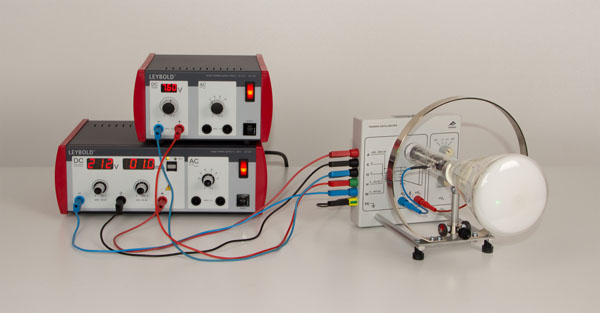
\includegraphics[width=0.8\linewidth]{./images/braun-tube.jpg}
  \caption{Montaje experimental.}
  \label{fig:set-up}
\end{figure}

Además, en una hoja milimetrada se marcó un punto de referencia, a partir del
cual se trazaron tres marcas adicionales a diferentes distancias.
Las posiciones relativas de estas marcas son las distancias entre el punto de
referencia y cada una de las marcas de \qty{1.5}{\centi m}, \qty{2.0}{\centi m}
y \qty{3.0}{\centi m}, respectivamente.

Se suministró una diferencia de potencial al cañón de electrones, generando un
haz de electrones que impactó en el extremo opuesto del tubo de vidrio cubierto
con un material fluorescente, lo que permitió observar un punto de luz.
Sobre este punto se posicionó la hoja milimetrada, de modo que el punto de
referencia coincidiera con el punto de luz y las otras tres marcas quedaran
alineadas debajo del mismo.

Posteriormente, se aplicó un potencial al capacitor, provocando la deflexión del
haz de electrones.
El valor del potencial se ajustó hasta que el punto de luz coincidiera con una
de las marcas en la hoja milimetrada, registrándose tanto la distancia como el
potencial aplicado.
A continuación, se suministró corriente a las bobinas de Helmholtz, ajustándose
para que el punto de luz deflectado volviera a su posición original, es decir,
al punto de referencia.
Este procedimiento se repitió para las tres marcas, y los valores de potencial
de aceleración utilizados fueron de \qty{390.0}{V}, \qty{445.6}{V} y \qty{523.0}{V}.


\section{Resultados y Análisis}
Utilizando el montaje descrito, se obtuvieron 22 conjuntos de datos
correspondientes a cinco potenciales de aceleración diferentes.
Con base en la \cref{eq:Campo_magnetico_enHaz}, se calculó el valor del campo
magnético generado por las bobinas de Helmholtz, mientras que con la
\cref{eq:carga-masa} se determinó la carga específica del electrón para cada caso.
Los resultados obtenidos se presentan en la \cref{tab:data}.

\begin{table}[htbp!]
	\centering
	\rowcolors{2}{white}{gray!25}
	\begin{tabular}{S[table-format=3.0(1)]|S[table-format=1.2(1)]|S[table-format=2.1(1)]|S[table-format=1.2(1)]|S[table-format=1.2(1)]}
		\toprule
		{$U \, (\unit{V})$} & {$I \, (\unit{A})$} & {$r \, (\unit{\centi m})$} &
			{$B \, (\unit{\milli T})$} & {$e/m \, (\unit{\tera C \per kg})$} \\
		\midrule
		153(1) & 1.03(1) & 08.8(1) & 0.60(1) & 0.11(4) \\
		153(1) & 1.52(1) & 07.9(1) & 0.89(1) & 0.06(2) \\
		153(1) & 2.00(1) & 05.5(1) & 1.17(1) & 0.07(2) \\
		153(1) & 2.52(1) & 04.5(1) & 1.47(1) & 0.06(2) \\
		201(1) & 1.03(1) & 09.2(1) & 0.60(1) & 0.13(5) \\
		201(1) & 1.51(1) & 06.3(1) & 0.88(1) & 0.13(5) \\
		201(1) & 2.00(1) & 04.9(1) & 1.17(1) & 0.12(4) \\
		201(1) & 2.53(1) & 04.0(1) & 1.48(1) & 0.11(4) \\
		250(1) & 1.02(1) & 10.4(1) & 0.60(1) & 0.13(4) \\
		250(1) & 1.51(1) & 07.0(1) & 0.88(1) & 0.13(5) \\
		250(1) & 2.01(1) & 05.2(1) & 1.17(1) & 0.13(5) \\
		250(1) & 2.50(1) & 04.2(1) & 1.46(1) & 0.13(5) \\
		300(1) & 1.02(1) & 10.4(1) & 0.60(1) & 0.15(5) \\
		300(1) & 1.50(1) & 08.0(1) & 0.88(1) & 0.12(4) \\
		300(1) & 2.03(1) & 05.8(1) & 1.19(1) & 0.12(4) \\
		300(1) & 2.50(1) & 05.0(1) & 1.46(1) & 0.11(3) \\
		300(1) & 3.00(1) & 04.7(1) & 1.75(1) & 0.08(2) \\
		350(1) & 1.02(1) & 12.5(1) & 0.60(1) & 0.12(3) \\
		350(1) & 1.48(1) & 08.8(1) & 0.87(1) & 0.12(3) \\
		350(1) & 2.02(1) & 06.6(1) & 1.18(1) & 0.11(3) \\
		350(1) & 2.51(1) & 05.3(1) & 1.47(1) & 0.11(3) \\
		350(1) & 3.03(1) & 04.5(1) & 1.77(1) & 0.11(3) \\
		\bottomrule
	\end{tabular}
	\caption{Valores para el campo magnético y la carga especifica.}
	\label{tab:data}
\end{table}

Los datos revelan una tendencia coherente con las predicciones teóricas,
permitiendo calcular un valor promedio para la relación carga-masa del electrón
de \(e/m =\qty{0.12(4)}{\tera C \per kg}\).
Al comparar este valor con el valor aceptado en la literatura de
\(e/m =\qty{0.176}{\tera C \per kg}\), se observó un error relativo porcentual
del \qty{9.09}{\percent}, considerando el límite superior del intervalo de
confianza.

La varianza de los datos, calculada en \num{0.229}, indica una dispersión
moderada en las mediciones, posiblemente atribuible a fluctuaciones en la
precisión instrumental y a la estabilidad del campo magnético.
A pesar de esta dispersión, el valor promedio obtenido es razonablemente cercano
al valor teórico, lo que sugiere que la metodología es adecuada para una
estimación aproximada de la relación carga-masa del electrón.

Sin embargo, para mejorar la precisión de los resultados, sería óptimo medir el
campo magnético de manera directa, en lugar de calcularlo a partir de la
corriente en las bobinas. Esto reduciría las posibles inexactitudes introducidas
por la dependencia del campo en factores como la geometría del sistema y la
homogeneidad del campo generado.


\section{Conclusiones}
Se logró determinar la carga específica del electrón, obteniendo un valor
promedio de \( e/m = \qty{0.12(4)}{\tera\C\per\kg} \), con un error del
\qty{9.09}{\percent} en comparación con los datos de la literatura usando el
limite superior del intervalo de confianza, y un error del \qty{31}{\percent}.
Además, se determinó el campo magnético generado por las bobinas para diferentes
valores de corriente.
Se observó que a mayor corriente, menor era el radio de la órbita, por que se
deduce un aumento en la fuerza magnética y el campo que la produce.


\printbibliography
\nocite{*}
\end{document}
